
\section{Estimulación eléctrica funcional}
La estimulación eléctrica funcional es la aplicación de corriente eléctrica a tejido excitable para suplementar o reemplazar funciones que se han perdido en individuos con daños neurológicos. El propósito de la intervención FES es habilitar funciones que se han perdido en individuos con daño al sistema nervioso mediante la sustitución o asistencia a las habilidades voluntarias de dichos individuos. En las aplicaciones FES la estimulación es requerida para lograr una función deseada, por lo tanto, los sistemas FES usualmente se diseñan para ser controlados a partir de señales relacionadas a la actividad o intención del propio usuario. Los dispositivos FES que son usados para sustituir una función neurológica que se ha perdido son comúnmente llamadas neuroprótesis \cite{Peckham2005}.

\section{Neuroprótesis}
Una neuroprótesis (NP) es un dispositivo que proporciona ráfagas cortas de impulsos eléctricos al sistema nervioso central o periférico a través de electrodos superficiales, para lograr producir funciones sensoriales o motoras. Estos dispositivos buscan sustituir o asistir una función dañada debido a una lesión o enfermedad en el sistema nervioso \cite{Popovic2008}\cite{Popovic2015}.

En general, existen dos tipos de neuroprótesis: a) las neuroprótesis autónomas, las cuales son sistemas autocontenidos que imitan las funciones de una contraparte biológica, y b) las neuroprótesis por comando, las cuales son sistemas que reemplazan o asisten una función sensitiva o motora que se ha perdido o disminuido. Estas últimas están compuestos por un sistema de control que interpreta la intención del usuario, utilizan sensores para detectar el estado del sistema, genera la activación del sistema motor o sensorial del usuario, y proporciona una retroalimentación al usuario \cite{Popovic2015}.

Las neuroprótesis motoras, las cuales son un ejemplo de NP por comando, son sistemas que asisten a personas que han sufrido algún tipo de lesión en la médula espinal o cerebro. Estas NP pueden actuar directamente en el sistema nervioso central, en el sistema nervioso periférico o bien en una combinación de ambos \cite{Popovic2015}.

\section{Señales de comando y retroalimentación}
Como se muestra en la Figura \ref{Figura: CompNeuroP}, una neuroprótesis por comando requiere de dos señales esenciales para lograr su correcto funcionamiento, una de estas es una señal de comando y otra es una señal de retroalimentación \cite{Popovic2015}.

\begin{figure}[htbp]
\centering
	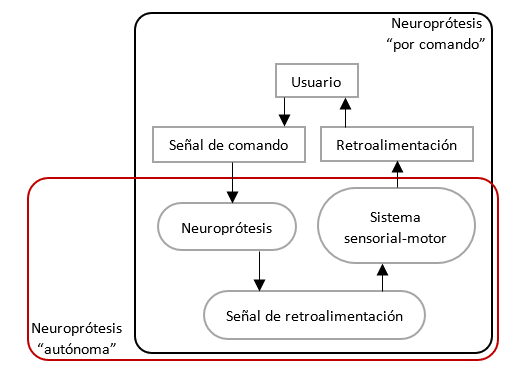
\includegraphics[scale=0.8]{CompNeuroP_ESP.png}
	\caption{Esquema de los componentes generales de una neuroprótesis autónoma y por comando. Adaptado de \cite{Popovic2015}.}
	\label{Figura: CompNeuroP}
\end{figure}

\subsection{Señal de comando}
Son señales utilizadas como indicadores de eventos de determinada tarea. En el caso de las neuroprótesis son las señales que controlan las acciones de esta, especialmente las acciones relacionadas a la estimulación eléctrica (inicio, fin, incremento de intensidad, disminución de intensidad, etc.).

\subsection{Señal de retroalimentación}
Es un tipo de señal que brinda al sistema información relacionada a la respuesta a un determinado comando. Estas señales, en el caso de las neuroprótesis, suelen estar relacionadas con el monitoreo del movimiento que está realizando el sujeto debido a los efectos de la estimulación eléctrica y pueden registrarse mediante distintos tipos de sensores.

\section{Esquemas de control}
Existen dos tipos de control importantes dentro de las aplicaciones de una neuroprótesis, los cuales se diferencian esencialmente en los tipos de señales que ocupan. En la Figura \ref{Figura: EsqCont} se ilustran a grandes rasgos las diferencias entre ambos esquemas de control \cite{Wright2016}.

\begin{figure}[htbp]
\centering
	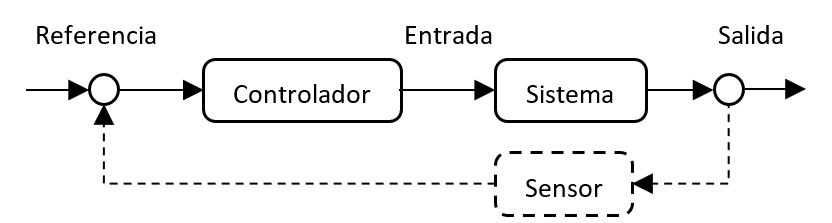
\includegraphics[scale=0.8]{EsquemasControl_ESP.png}
	\caption{Esquema general de control en lazo abierto y control en lazo cerrado. El control en lazo abierto se ilustra con una línea sólida. El control en lazo cerrado se lleva a cabo cuando se incluye el elemento sensor, el cual se ilustra con una línea discontinua. Adaptado de \cite{Wright2016}.}
	\label{Figura: EsqCont}
\end{figure}

\subsection{Control en lazo abierto}
En el control en lazo abierto se genera un comando a la línea de base, esperando que este comando produzca la salida correcta. Aquí no existe una medición de la salida generada, por lo cual tampoco existe alguna medición del error que pudiera utilizarse como mecanismo para la modulación del comando que se genera \cite{Wright2016}.

\subsection{Control en lazo cerrado}
El control en lazo cerrado requiere de la inclusión de algún elemento sensor en el sistema que se desea controlar. Este control retroalimentado genera un comando a la línea de base y el elemento sensor mide la salida de la planta en respuesta al comando. Esta medición de la salida puede utilizarse para determinar diferencias entre la salida esperada y la real, generando así una señal de error que puede utilizarse como retroalimentación hacia el controlador para realizar modificaciones en los comandos generados \cite{Wright2016}.

Dichos esquemas de control suelen utilizar algunas de las siguientes políticas de control:
\begin{itemize}
	\item Control bang-bang (control On-Off): es una política de control en la que cuando una variable cruza un umbral predefinido, se activa un programa que habilita o deshabilita determinadas funciones del esquema de control \cite{Wright2016}.
	\item Máquina de estados finitos: es un modelo de sistema que puede considerarse como una implementación más compleja de la política On-Off. En este modelo, la medición de una variable del sistema en combinación con el estado actual desencadena una serie de acciones y una transición de estado. Este tipo de modelo es periódico, entonces pueden realizarse transiciones de estado en respuesta al tiempo \cite{Wright2016}.
\end{itemize}

{\color{red}AGREGAR CONTROLES PID}\\
{\color{blue}Enrique: ¿debería agregar algo sobre la conversión de números binarios en complemento 2?}

%\section{\color{blue}Números binarios}


%\subsection{Complemento a uno}


%\subsection{Complemento a dos}


%\subsection{Conversión complemento a dos a binario}
